\chapter{Phase du projet --- Distribution des tâches}
\newpage

\section{Contexte}
Le projet repose, en assez grande partie, sur des domaines qu’il nous
fallait découvrir et étudier. C’est pourquoi l’attribution et la définition
des tâches à été une problématique importante dans le projet lockatme.
Cette étape est essentielle pour le bon déroulement du développement.
Nous nous sommes efforcés d’attribuer les tâches à des duos ou trios afin de
permettre deux choses : une auto-formation étant parfois nécessaire, les
membres assignés à une même tâche pouvaient partager les connaissances et les
difficultés, afin de faire avancer le développement plus vite. De plus les
membres ne devraient pas rester bloquer sur une tâche étant donné que les
attributions se font en fonction des compétences de chacuns.

\section{Listes des tâches}
La liste des tâches est fortement susceptible d’évoluer au cours du projet en
fonction de l’évolution de celui-ci, des difficultés recontrées et du temps
imparti. La réalisation des tests n’est pas spécifiée dans cette liste.
Niveaux d’importances: 1 - essentiel, 2 - important, 3 - importance modérée,
4 - optionnel.

\vspace{0.5cm}

T1 : Cahier des charges (1)
\begin{itemize}
  \item{conception}
  \item{rédaction}
  \item{validation}
\end{itemize}

T2 : Déverrouillage
\begin{itemize}
  \item{algo reconnaissance faciale (1)}
  \item{algo déverrouillage par mot de passe (1)}
  \item{gestion des cas d’erreurs (1)}
  \item{fichier configuration/personnalisation (2)}
\end{itemize}

T3 : Implementation système, installation
\begin{itemize}
  \item{verrouillage écran (1)}
  \item{déverrouillage écran (1)}
  \item{installation qualification (2)}
  \item{upload du logiciel sur des dépôts standards}
  \item{readme (2)}
\end{itemize}

T4 : Amélioration
\begin{itemize}
  \item{interface graphique (3)}
  \item{développemement plateforme commune de verrouillage/déverrouillage
        d’écran (4)}
\end{itemize}

\section{Repartition des tâches}

Du fait de la disparité des compétences du groupe, il était essentiel
d'associer plusieurs personnes à chaque tâche. Afin de faciliter le travail
mais aussi pour que chacuns apprennent de nouvelles choses. Comme dis plus haut
nous avons donc
décider d'attribuer chaque sous-tâche à des duos ou trios; composés d'une
personne référente et d'une personne peu ou pas expérimenté dans le domaine
ciblé. Ainsi la personne ayant plus de connaissance est capable de diviser
le travail en d'autres sous-tâches (non présente sur le diagramme) afin de faire
participer au mieux les autres membres.

Nous avons prit soin d'associer les tâches bloquantes aux personnes
compétentes. De plus si une difficulté survient sur une tâche,
les réunions hebdomadaires permettent de faire le point et d'aider la
personne.

\section{Diagramme de Gantt}
Voici le diagramme de Gantt résumant les principales tâches et sous-tâches
ainsi que la repartition de celles-ci.
\\
\\
\begin{figure}[h]
  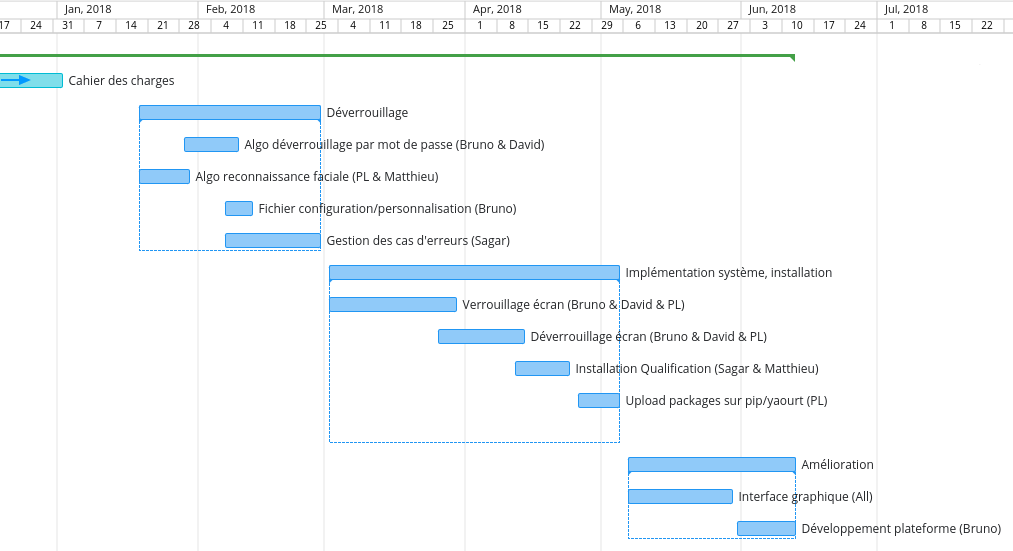
\includegraphics[width=\linewidth]{gantt}
  \caption{diagramme de Gantt}
\end{figure}
